\newpage
\section{Entity-Relationship Model}
Steps of Database Design
\begin{enumerate}\small
    \item Requirement analysis
    \subitem What data, applications, and operations needed.
    \item Conceptual database design
    \subitem A high-level description of data, constraints using\\ Entity-Relationship (E-R) model
    or a similar high level data model.
    \item Logical database design
    \subitem Convert the conceptual design into a DB schema.
    \item Schema refinement
    \subitem Normalization of relations: Check relational s- chema for redundancies and related
    anomalies.
    \item Physical database design
    \subitem Indexing, query, clustering, and database tuning.
    \item Create and initialize the database \& Security design
    \subitem Load initial data, testing.
    \subitem Identify different user groups and their roles.
\end{enumerate}

\subsection{Entity Sets}
\subsubsection{Entity}
The real world can be modeled as:
\begin{itemize}\small
    \item A collection of entities (实体)
    \item Relationships (联系) among entities
\end{itemize}

An entity is an object that exists and is distinguishable from other objects. --- An entity may be concrete, or abstract.

Entities have attributes (属性). 

An entity set is a set of entities of the same type that share the same properties.

\subsubsection{Attributes}
An entity is represented by a set of attributes, that is descriptive properties possessed by all members of an entity set. Domain (域, value set) is the set of permitted values for each attribute.

Attribute types:
\begin{enumerate}\small
    \item Simple and composite attributes (简单和复合属性,如sex, name).
    \item Single-valued and multi-valued attributes(单值和多值属性).
    \subitem E.g., multivalued attribute: phone-numbers (多个电话号码).
    \item Derived attributes (派生属性).
    \subitem Can be computed from other attributes, e.g., age, given date of birth.
    \subitem versus base attributes or stored attributes (基属性,存储属性).
\end{enumerate}

\subsubsection{Composite Attributes}
\begin{figure}[H]
    \centering
    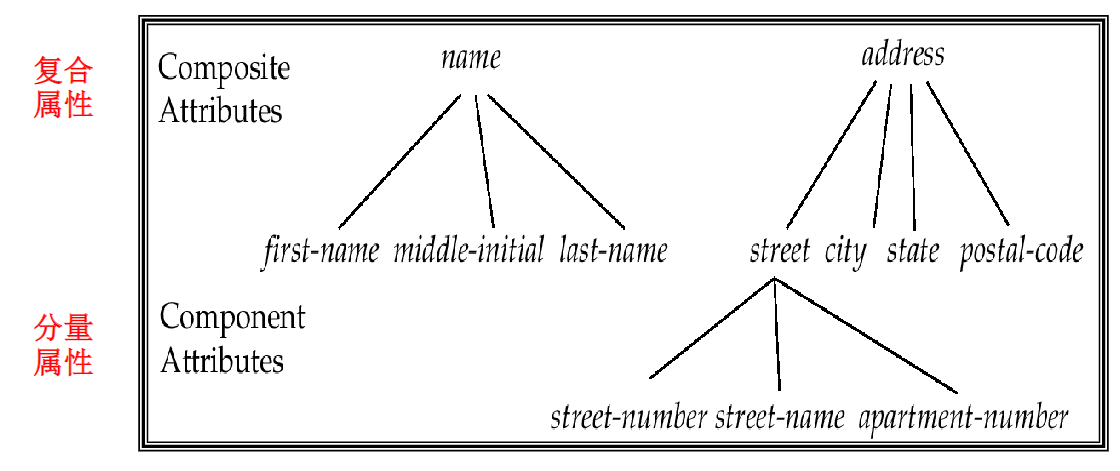
\includegraphics[width=0.479\textwidth]{DB5/Composite Attributes}
    \caption{Composite Attributes}
\end{figure}


\subsection{Relationship Sets}
A relationship is an association among several entities (是二个或多个不同类实体之间的关联). A relationship set is a set of relationship of the same type. 

\begin{definition}
    A relationship set is a mathematical relation among $n\ge 2$ entities, each taken from entity sets
    \begin{align*}
        \left\{ (e_1, e_2, \dots, e_n)  | e_1 \in E_1, e_2 \in E_2, \dots, e_n \in E_n \right\}
    \end{align*}
    where $(e_1, e_2, \dots, e_n)$ is a relationship, $E_i$ is an entity set. 
\end{definition}

\subsubsection{Degree of a Relationship Set}
Refers to the number of entity sets that participate in a relationship set.
\begin{enumerate}
    \item Relationship sets that involve two entity sets are binary (or degree two).
    \item Relationships between more than two entity sets are rare. Most relationships are binary. (More on this later.)
\end{enumerate}

\subsubsection{Mapping Cardinalities}
Express the number of entities to which another entity can be associated via a relationship set. (一个 联系集 中,一个实体可以与另一类实体相联系的实体数目。其中数目是指最多一个还是多个)

Most useful in describing binary relationship sets. For a binary relationship set the mapping cardinality must be one of the following types:
\begin{itemize}\small
    \item One to one (1 : 1)
    \item One to many (1 : n)
    \item Many to one (n : 1)
    \item Many to many (n : m)
\end{itemize}

Note: Some elements in entity set A and B may not be mapped to any elements in the other set.


\subsection{Keys}
\subsubsection{Keys for Entity Sets}
\begin{enumerate}
    \item A super key of an entity set is a set of one or more attributes whose values uniquely determine each entity. 
    \item A candidate key of an entity set is a minimal super key. 
    \item Although several candidate keys may exist, one of the candidate keys is selected to be the primary key.
\end{enumerate}

\subsubsection{Keys for Relationship Sets}
The combination of primary keys of the participating entity sets forms a super key of a relationship set (参与一个联系集的各实体集的码的组合,构成该联系集的超码). Must consider the mapping cardinality of the relationship set when deciding what are the candidate keys (1:1, 1:n, m:n). Need to consider semantics of relationship set in selecting the primary key in case of more than one candidate key. 

\subsection{E-R Diagram}

\begin{figure}[H]
    \centering
    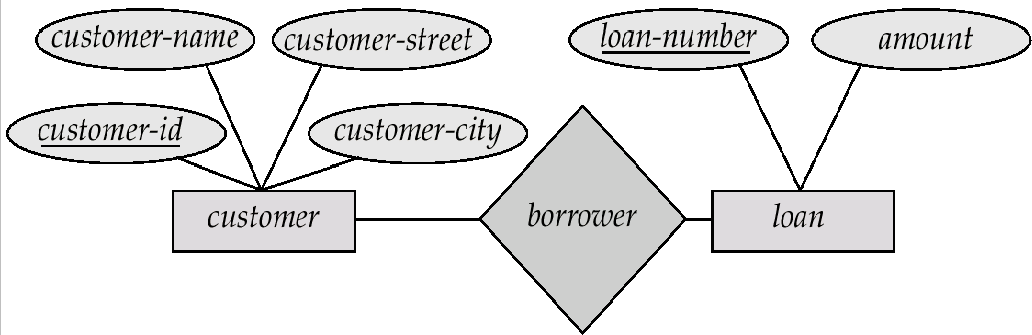
\includegraphics[width=0.479\textwidth]{DB5/E-R Diagrams}
    \caption{E-R Diagrams}
\end{figure}

\begin{itemize}\small
    \item Rectangles represent entity sets.
    \item Diamonds represent relationship sets.
    \item Lines link attributes to entity sets and entity sets to relationship sets.
    \item Ellipses represent attributes.
    \subitem Double ellipses represent multivalued attributes.
    \subitem Dashed ellipses denote derived attributes.
    \item Underline indicates primary key attributes (will study later).
\end{itemize}

\begin{figure}[H]
    \centering
    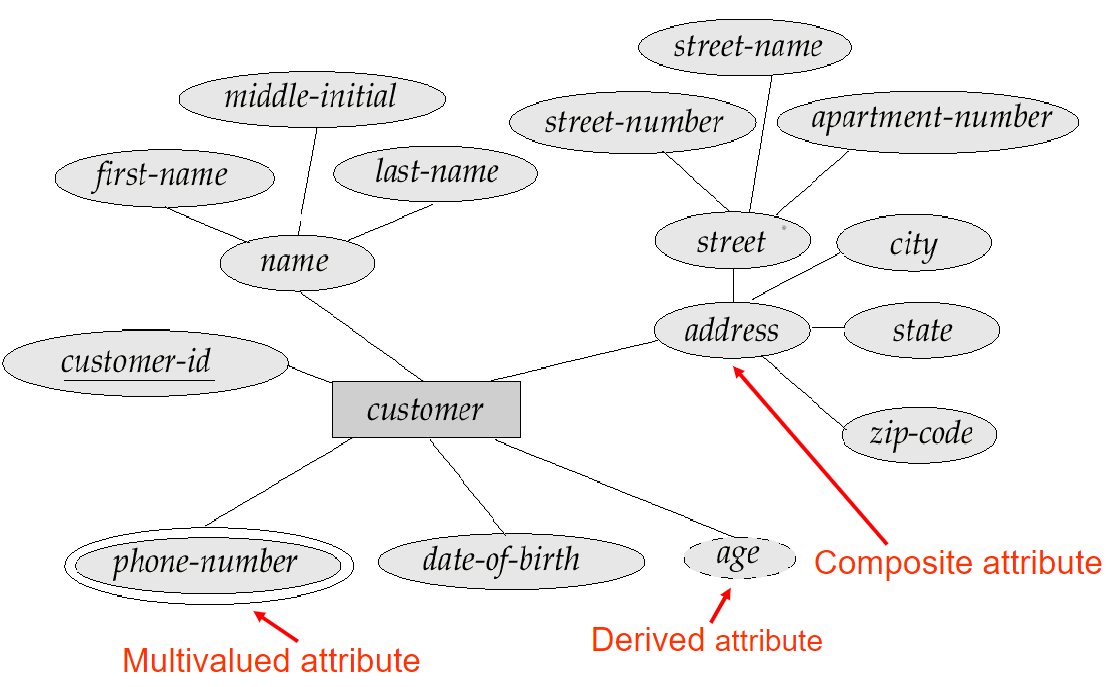
\includegraphics[width=0.479\textwidth]{DB5/E-R Diagram With Composite, Multivalued and Derived Attributes}
    \caption{E-R Diagram With Composite, Multivalued and Derived Attributes}
\end{figure}

Role: the function that an entity plays in a relationship. Role labels are optional, and are used to clarify semantics of the relationship.

\begin{figure}[H]
    \centering
    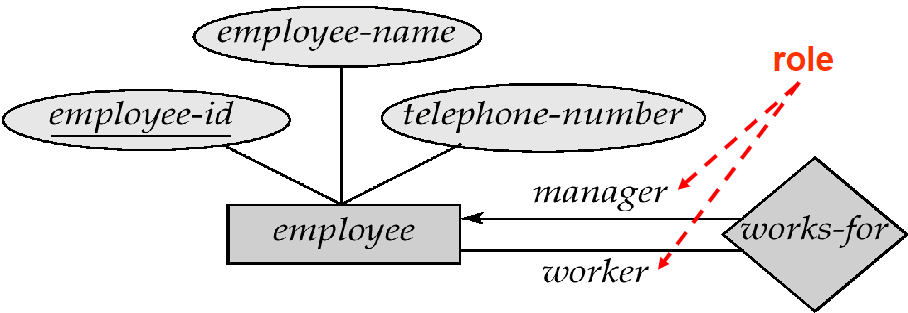
\includegraphics[width=0.309\textwidth]{DB5/Role}
    \caption{Role}
\end{figure}

\subsubsection{Express the Cardinality Constraints}
We express cardinality constraints by drawing either a directed line ($\rightarrow$), signifying ``one'', or an undirected line (---), signifying ``many'', between the relationship set and the entity set.

\subsubsection{Participation of an Entity Set in a Relationship Set}
\begin{itemize}
    \item Total participation (全参与) (indicated by double line): every entity in the entity set participates in at least one relationship in the relationship set.
    \item Partial participation (部分参与): some entities may not participate in any relationship in the relationship set.
\end{itemize}

映射基数约束(Mapping cardinality constraints),限定了一个实体与发生关联的另一端实体可能关联的数目上限。

全参与和部分参与约束,则反映了一个实体参与关联的数目下限: 0次,还是至少1次。

\begin{figure}[H]
    \centering
    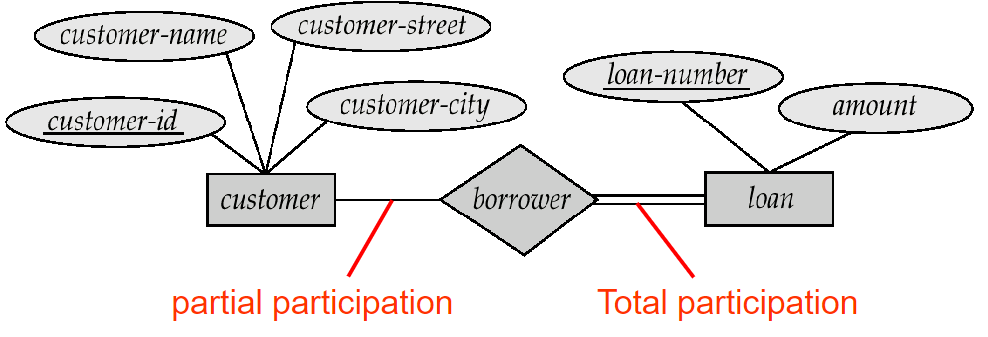
\includegraphics[width=0.479\textwidth]{DB5/Participation}
    \caption{Participation}
\end{figure}


\subsubsection[Alternative Notation for relationship Constraints]{Alternative Notation for relationship Constr- aints}
Alternative notation for cardinality constraints and participation constraints.

E.g., 一个客户可以借多笔或0笔贷款, 一笔贷款至少、至多属于一个客户. 

\begin{figure}[H]
    \centering
    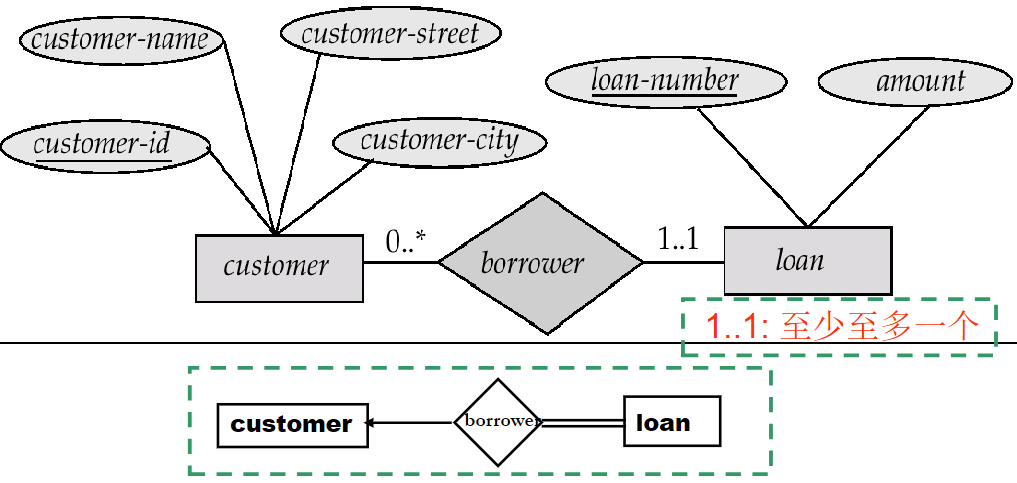
\includegraphics[width=0.479\textwidth]{DB5/Alternative Notation}
    \caption{Alternative Notation}
\end{figure}


\subsubsection{E-R Diagram with a Ternary Relationship}
一个银行职员在多个支行兼职, 并承担不同类型的工作. 
\begin{figure}[H]
    \centering
    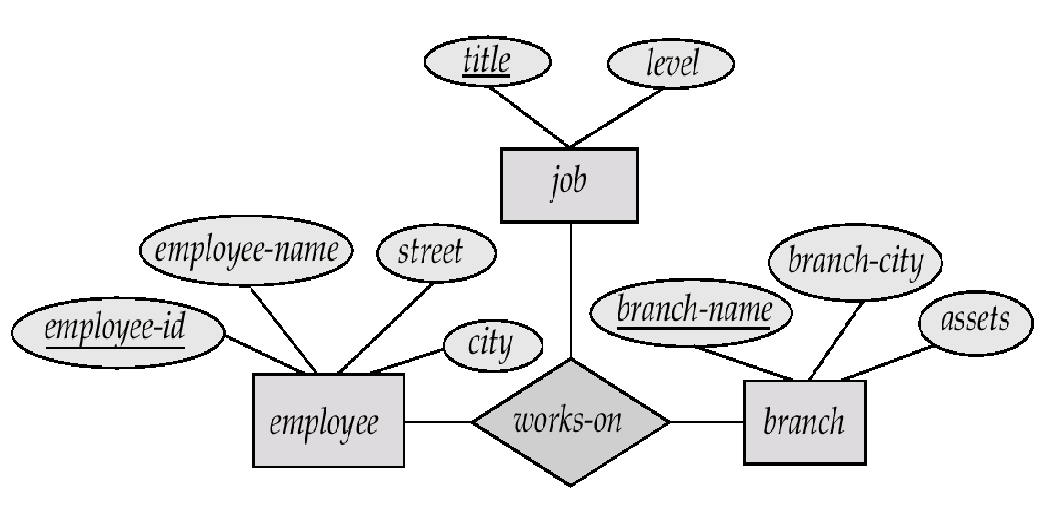
\includegraphics[width=0.479\textwidth]{DB5/E-R Diagram with a Ternary Relationship}
    \caption{E-R Diagram with a Ternary Relationship}
\end{figure}


\subsubsection{Binary vs. Non-Binary Relationships}
Some relationships that appear to be non-binary may be better represented using binary relationships. Using two binary relationships allows partial information. But there are some relationships that are naturally non-binary. 

\subsubsection[Converting Non-Binary Relationsh- ips to Binary Form]{Converting Non-Binary Relationships to Binary Form}
In general, any non-binary relationship can be represented using binary relationships by creating an artificial entity set. 

\begin{enumerate}
    \item Replace non-binary relationship $R$ between entity sets $A$, $B$, and $C$ by an entity set $E$, and three new relationship sets.
    \item Create a special identifying attribute for $E$.
    \item Add any attributes of $R$ to $E$.
    \item For each relationship $(a_i,\ b_i,\ c_i)$ in $R$, create $R_A,\ R_B,\ R_C$. 
\end{enumerate}

\begin{figure}[H]
    \centering
    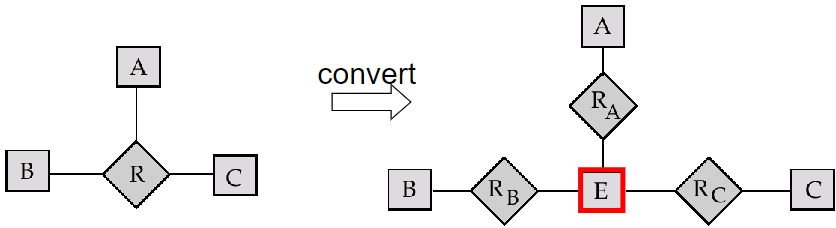
\includegraphics[width=0.489\textwidth]{DB5/Converting}
    \caption{Converting}
\end{figure}


\subsection{Weak Entity Sets}
An entity set that does not have a primary key is referred to as a weak entity set (弱实体集).

The existence of a weak entity set depends on the existence of a identifying entity set or owner entity set (标识实体集或属主实体集). 

The related relationship is called identifying relationship (标识性联系). 

The discriminator or partial key (分辨符或部分码) of a weak entity set is the set of attributes that distinguishes among all those entities in a weak entity set that depend on one particular strong entity. The primary key of a weak entity set is formed by the primary key of the strong entity set on which the weak entity set is existence dependent, plus the weak entity set’s discriminator.

Note: the primary key of the strong entity set is not explicitly stored with the weak entity set, since it is implicit in the identifying relationship. 

\begin{figure}[H]
    \centering
    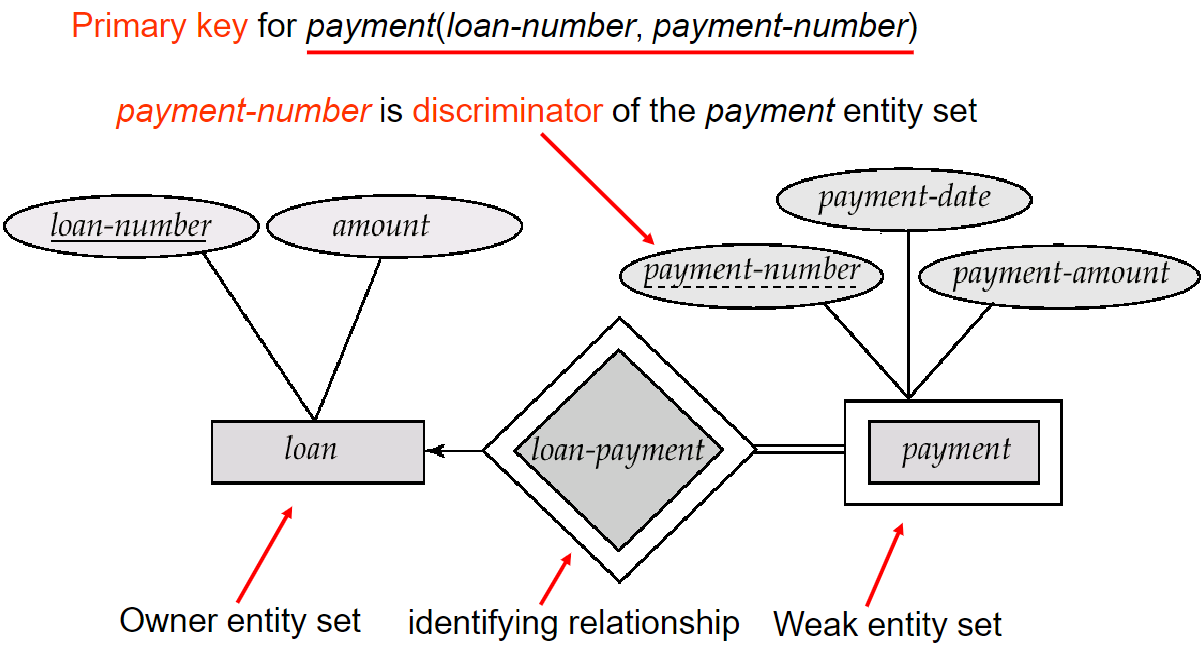
\includegraphics[width=0.479\textwidth]{DB5/Weak Entity Sets}
    \caption{Weak Entity Sets}
\end{figure}


\subsection{Extended E-R Features}
Stratum of the entity set:
\begin{enumerate}
    \item Specialization (特殊化、具体化): Top-down design process
    \begin{figure}[H]
        \centering
        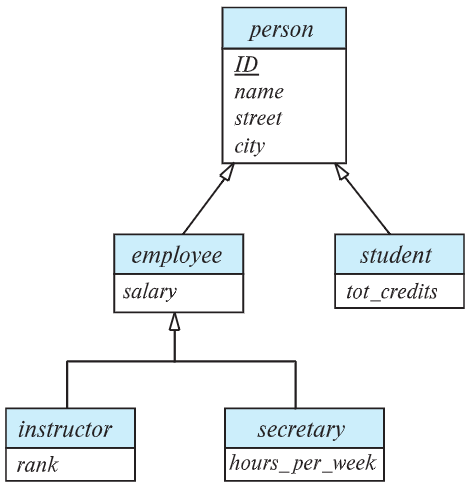
\includegraphics[width=0.179\textwidth]{DB5/Specialization}
        \caption{Specialization Example}
    \end{figure}
    
    \item Generalization (泛化、普遍化): Bottom-up design process
\end{enumerate}

\subsubsection{Design Constraints on a Specialization / Generalization}
\begin{enumerate}
    \item Constraint on which entities can be members of a given lower-level entity set.
    \begin{itemize}\small
        \item Condition-defined (条件定义的)
        \item User-defined
    \end{itemize}
    
    \item Constraint on whether or not entities may belong to more than one lower-level entity set within a single generalization.
    \begin{itemize}\small
        \item Disjoint (不相交)
        \subitem An entity can belong to only one lower-level entity set.
        \subitem Noted in E-R diagram by writing disjoint next to the ISA triangle.
        \item  Overlapping (可重叠)
        \subitem An entity can belong to more than one lower-level entity set.
    \end{itemize}
    
    \item Completeness constraint (完全性约束) -- specifies whether or not an entity in the higher-level entity set must belong to at least one of the lower-level entity sets within a generalization.
    \begin{itemize}\small
        \item Total: an entity must belong to one of the lower-level entity sets.
        \item Partial: an entity need not belong to one of the lower-level entity sets.
    \end{itemize}
\end{enumerate}

\subsubsection{Aggregation}
Eliminate this redundancy via aggregation.
\begin{itemize}\small
    \item Treat relationship as an abstract entity.
    \item Allows relationships between relationships.
    \item Abstraction of relationship into new entity.
\end{itemize}

\subsubsection{Summary of Symbols Used in E-R Notation}
\ref{E-R Notation}

\begin{figure*}[htb]
    \centering
    \begin{subfigure}{0.48\textwidth}
        \centering
        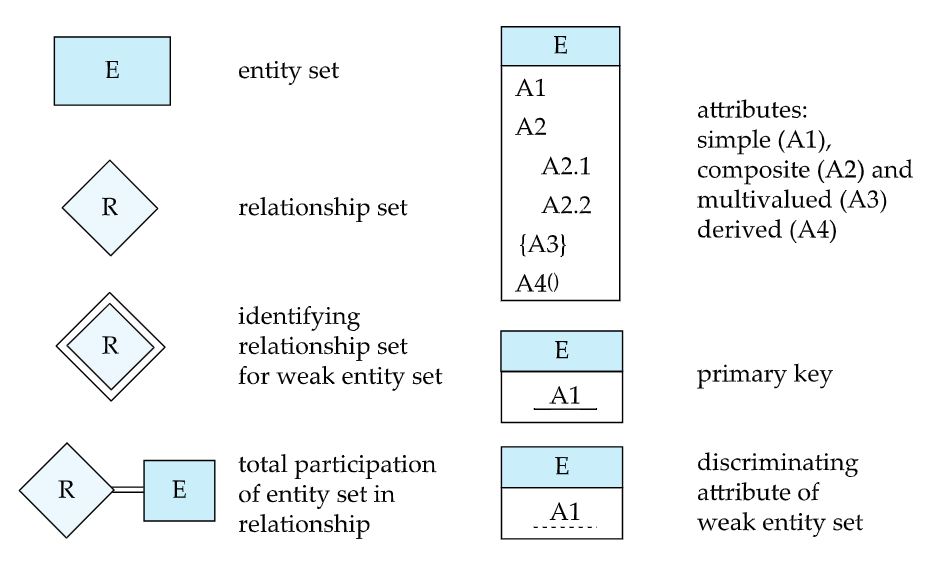
\includegraphics[width=\textwidth]{DB5/E-R Notation1}
    \end{subfigure}
    \begin{subfigure}{0.48\textwidth}
        \centering
        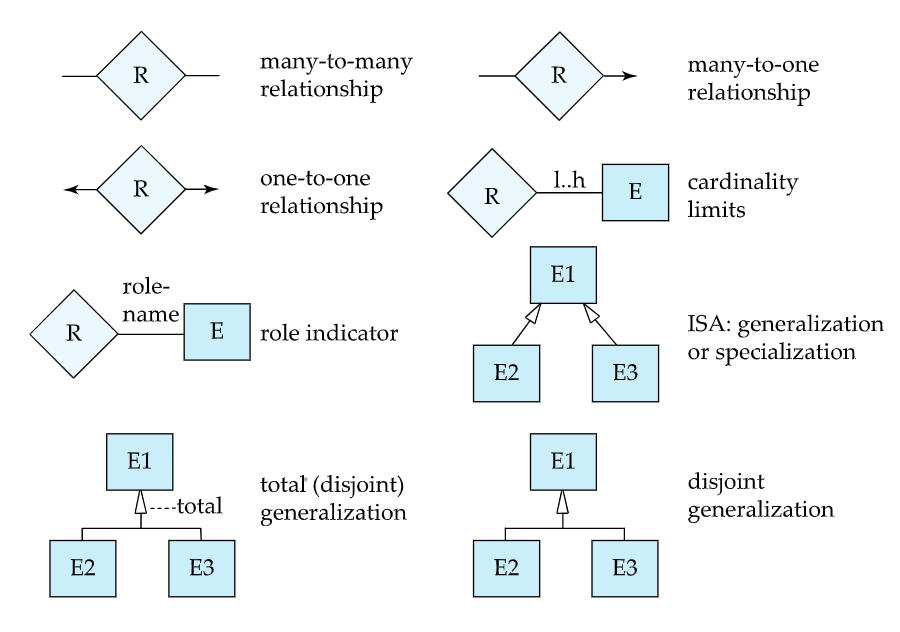
\includegraphics[width=\textwidth]{DB5/E-R Notation2}
    \end{subfigure}
    \caption{E-R Notation}
    \label{E-R Notation}
\end{figure*}




\subsection{Design of an E-R Database Schema}
\subsubsection{E-R Design Decisions}
\begin{enumerate}
    \item Use an attribute or entity set to represent an object?
    \subitem 若一个对象只对其名字及单值感兴趣,则可作为属性,如性别;若一个对象除名字外,本身还有其他属性需描述,则该对象应定义为实体集。如电话, 部门. 
    \subitem 一个对象不能同时作为实体和属性. 
    \subitem 一个实体集不能与另一实体集的属性相关联,只能实体与实体相联系. 
    \item Use it as an entity set or a relationship set?
    \subitem Relationship set --- to describe an action that occurs between entities (二个对象之间发生的动作 --- 用``relationship set''表示).
    \subitem The mapping cardinality will effect the matter.
    \item Use it as an attribute of an entity or a relationship?
    \subitem 要从对象的语义独立性和减少数据冗余方面考虑
    \item The use of a ternary or n-ary relationship versus a pair of binary relationships.
    \item The use of a strong or weak entity set. 
    \item The use of specialization/generalization --– contributes to modularity in the design (有助于模块化). 
    \item The use of aggregation –-- can group a part of E-R diagram into a single entity set, and treat it as a single unit without concern for the details of its internal structure.
\end{enumerate}

\subsection{Reduction of an E-R Schema to Tables}
Converting an E-R diagram to a table format is the basis for deriving a relational database design from an E-R diagram.

\subsubsection{Entity Sets}
\begin{enumerate}
    \item Entity Set with Composite Attributes: Composite attributes are flattened out by creating a separate attribute for each component attribute.
    \item Entity Set with Multivalued Attributes: A multivalued attribute M of an entity E is represented by a separate table EM. Each value of the multivalued attribute maps to a separate row of the table EM. 
    \item Representing Weak Entity Sets: A weak entity set becomes a table that includes a column for the primary key of the identifying strong entity set.
\end{enumerate}



\subsubsection{Representing Relationship Sets as Tables}
A relationship set is represented as a table with columns for the primary keys of the two participating entity sets, (which are foreign keys here) and any descriptive attributes of the relationship set itself.

\begin{enumerate}\small
    \item tables for many to many relationship sets: The two attributes corresponding to the two entity sets become the primary key of the table.
    \item tables for many to one relationship sets: The attribute corresponding to the entity set on the “many” side becomes the primary key of the table. 
    \item tables for one to one relationship sets: like 2)
\end{enumerate}

\subsubsection{Redundancy of Tables}
\begin{enumerate}\small
    \item Many-to-one and one-to-many relationship sets that are total on the many-side can be represented by adding an extra attribute to the “many” side, containing the primary key of the one side (对1:n联系, 可将“联系”所对应的表,合并到对应“多”端实体的表中).
    \subitem If participation is partial on the many side, replacing a table by an extra attribute in the relation corresponding to the “many” side could result in null values. 
    \subitem For one-to-one relationship sets, either side can be chosen to act as the “many” side.  That is, extra attribute can be added to either of the tables corresponding to the two entity sets. 
    \item The table corresponding to a relationship set linking a weak entity set to its identifying strong entity set is redundant (联系弱实体集及其标识性实体集的联系集对应的表是冗余的,即对应identifying relationship的表是多余的。).
\end{enumerate}

\subsubsection{Representing Specialization as Tables}
\begin{itemize}
    \item Method 1
    \begin{enumerate}
        \item Form a table for the higher level entity.
        \item  Form a table for each lower level entity set, including primary key of higher level entity set and local attributes.
        \item Drawback: getting information about. 
    \end{enumerate}
    \item Method 2
    \begin{enumerate}
        \item Form a table for each entity set with all local and inherited attributes. 
        \item If specialization is total, table for generalized entity not required to store information. 
        \item Drawback: Attributes may be stored redundantly       
    \end{enumerate}
\end{itemize}